\section{Ground Motion Waveforms}
\label{sec:ims}

Fundamental to the use of the GMPE-SMTK is the strong motion waveform. For the widest portability we adopt the simplest representation of the waveform in the toolkit, which requires only the acceleration and the time steps. As seen in the previous chapter, the strong motion database stores the acceleration, velocity and displacement trace. 

\textbf{The conventional units for acceleration, velocity and displacement waveforms in the GMPE-SMTK are ``cm/s/s'', ``cm/s'' and ``cm'' respectively.}

The GMPE-SMTK contains two tools for extracting basic information and common ground motion intensity measures from single waveforms, or from a horizontal pair of waveforms: \verb=intensity_measures= and \verb=response_spectrum=. To use them in an application we can import them as follows:

\begin{python}[frame=single]
import smtk.intensity_measures as ims
import smtk.response_spectrum as rsp
\end{python}

This will load two objects into the workspace \verb=ims= (the intensity measure tools) and \verb=rsp= (the response spectrum tools)

In most applications we assume it is the acceleration time series that is available. In the following example we consider a pair of strong motion records, where each record is represented by a simple ascii (text) file:\verb=sm_record_x.txt= and \verb=sm_record_y.txt=. The timestep of each record is 0.002 s.

\begin{python}[frame=single]
# Import the numpy tools
import numpy as np
# Load in the records
accel_x = np.genfromtxt("sm_record_x.txt")
accel_y = np.genfromtxt("sm_record_y.txt")
time_step = 0.002
\end{python}

Once loaded the user can retrieve the velocity and displacement time-series, calculated using double integration of the acceleration time series. A simple tool to do this is found in the \verb=ims= tools:

\begin{python}[frame=single]
vel_x, disp_x = ims.get_velocity_displacement(accel_x,
                                              time_step,
                                              units="cm/s/s") 
\end{python}

\noindent where \verb=units= is the units of the uploaded record. 

\noindent The first steps one might wish to take when analysing a strong motion record is to look at the waveforms. To do this we make use of the simple tool inside the response spectrum package called \verb=plot_time_series=.
This can be called as follows for the x=component of the pair:

\begin{python}[frame=single]
rsp.plot_time_series(accel_x,
                     time_step,
                     velocity=vel_x,
                     displacement=disp_x,
                     units="cm/s/s",
                     filename="path/to/output/image.eps",
                     filetype="eps",
                     dpi=300,
                     linewidth=1.5) 
\end{python}

This command would produce a plot of the style shown in Figure \ref{fig:time_series}.

\begin{figure}[htb]
	\centering
		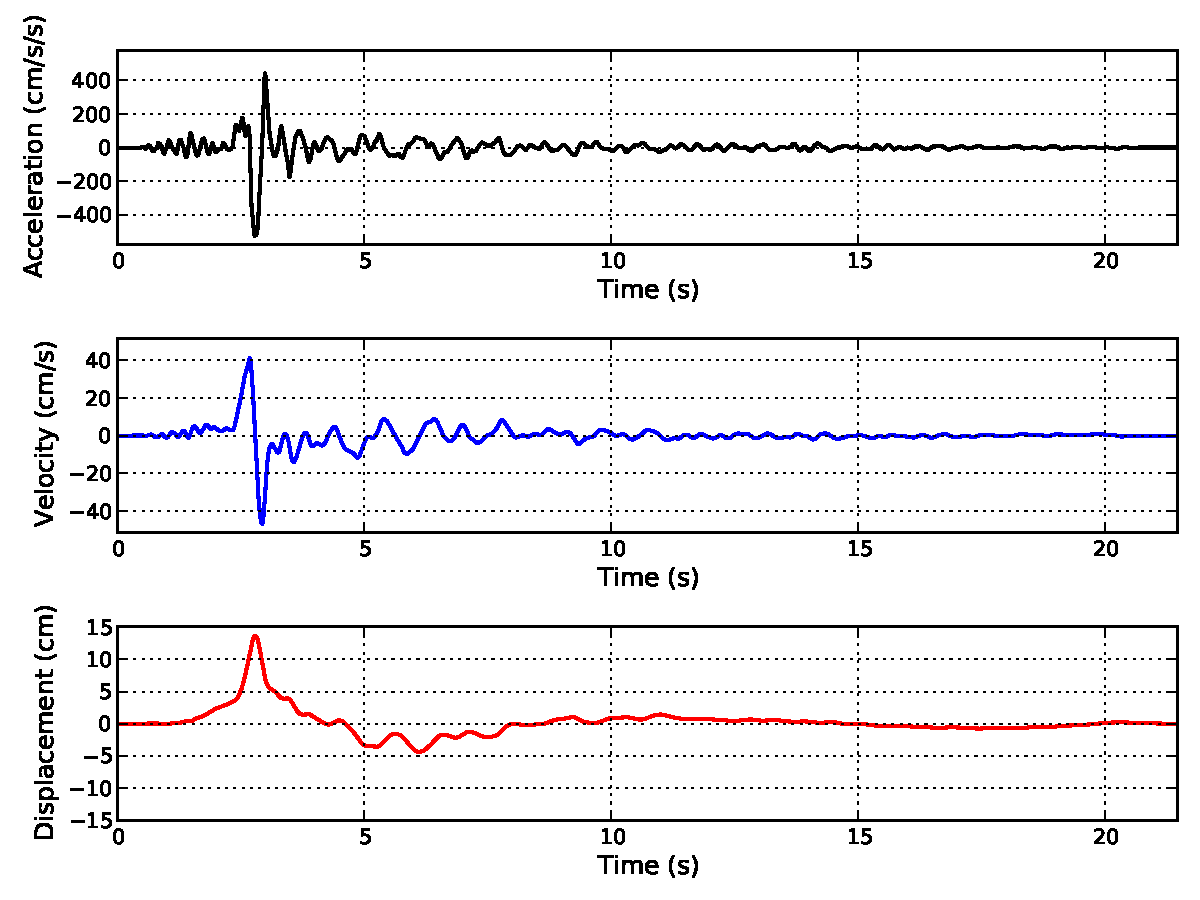
\includegraphics[height=8cm, keepaspectratio=true]{./figures/ims/timeseries_plot1.pdf}
	\caption{Example time series for a single record: acceleration (top), velocity (middle) and displacement (bottom)}
	\label{fig:time_series}
\end{figure}

\noindent The function \verb=plot_time_series= requires two essential arguments: 
\begin{itemize}
\item \verb=acceleration=: The acceleration time series
\item \verb=time_step=: The time step of the acceleration time series
\end{itemize}

\noindent If the user already has the velocity and displacement time series available these can be input with the following keyword arguments:

\begin{itemize}
\item \verb=velocity=: The velocity time series (cm/s), which will be calculated if not provided.
\item \verb=displacement=: The time step of the displacement (cm) time series, which will be calculated if not provided.
\item \verb=units=: The units of the acceleration time series (defaults to ``cm/s/s'')
\item \verb=figure_size=: The internal size of the figure (defaults to $(8, 6)$)
\item \verb=filename=: The name of the file to which the figure will be saved (if desired, by default it is ``None'')
\item \verb=filetype=: The format of the output file (default=``png'').
\item \verb=dpi=: Resolution (dots per inch) of the output figure (default = 300)
\item \verb=linewidth=: The thickness (point size) of the lines (default = 1.5)
\end{itemize}


\section{Scalar Intensity Measures}
\label{sec:scalar_ims}

\subsection{Peak Measures}

The following describes the simple ``peak'' measures, peak ground acceleration (PGA), peak ground velocity (PGV) and peak ground displacement (PGD), that can be extracted from the record:
\begin{align}
PGA = \max |a \left( t \right)| \nonumber\\
PGV = \max |v \left( t \right)| \\
PGD = \max |d \left( t \right)| \nonumber
\end{align}
where $a \left( t \right)$, $v \left( t \right)$ and $d \left( t \right)$ are the acceleration, velocity and displacement time series respectively.

These values can all be extracted by one function in the \verb=ims= tool named \verb=get_peak_measures=. These values can be called as follows:

\begin{python}[frame=single]
pga, pgv, pgd, vel_x, disp_x = get_peak_measures(time_step,
                                                 accel_x,
                                                 get_vel=True,
                                                 get_disp=True)
\end{python}

\noindent This function returns the three peak measures as well as the velocity and displacement (if required). The keywords \verb=get_vel= and \verb=get_disp= will, when set to \verb=True=, calculate velocity and displacement.

\subsection{Duration}
\subsection{Other Scalar Measures}

\section{Response Spectra}
\label{sec:response_spectra}

The response spectrum is one of the most important elements of a ground motion record used in earthquake engineering. The response spectrum provides the peak responses of a set a single-degree-of-freedom (SDOF) oscillators with different natural periods ($T$), and damping ratio $\xi$. The pseudospectral acceleration at a given period $Sa \left({T, \xi} \right)$, and its corresponding pseudospectral velocity and displacements, $Sv \left( {T, \xi} \right)$ and $Sd \left( {T, \xi} \right)$ respectively, are the most widely used means to characterise the ground motion input for a given structure. In addition to the peak values however, it is also useful to have available the acceleration, velocity and displacement response time series of the SDOF oscillators for each natural period. The GMPE-SMTK response spectra tools are designed to return the most comprehensive set of information to describe the SDOF response for each record.

To calculate a response spectrum for a record, two response spectra calculators are currently available: ``Newmark-$\beta$'' and ``Nigam \& Jennings'' (\cite{NigamJennings1969}).

These can be called following the process below:
\begin{python}
# Define the periods for calculating spectral acceleration
periods = np.array([0.01, 0.02, 0.03, 0.04, 0.05, 0.075, 0.1, 
                    0.11, 0.12, 0.13, 0.14, 0.15, 0.16, 0.17, 
                    0.18, 0.19, 0.20, 0.22, 0.24, 0.26, 0.28,
                    0.30, 0.32, 0.34, 0.36, 0.38, 0.40, 0.42,
                    0.44, 0.46, 0.48, 0.50, 0.55, 0.6-, 0.65,
                    0.70, 0.75, 0.80, 0.85, 0.90, 0.95, 1.00,
                    1.10, 1.20, 1.30, 1.40, 1.50, 1.60, 1.70, 
                    1.80, 1.90, 2.00, 2.20, 2.40, 2.60, 2.80, 
                    3.00, 3.20, 3.40, 3.60, 3.80, 4.00, 4.20,
                    4.40, 4.60, 4.80, 5.00, 5.50, 6.00, 6.50, 
                    7.00, 7.50, 8.00, 8.50, 9.00, 9.50, 10.0])
# Call the Newmark-Beta methodology
newmark_beta = rsp.NewmarkBeta(acceleration,
                               time_step,
                               periods,
                               damping=0.05,
                               units="cm/s/s")

spectra, time_series, acc, vel, dis = newmark_beta.evaluate()

# Call the Nigam & Jennings (1969) method
nigam_jennings = rsp.NigamJennings(acceleration,
                                   time_step,
                                   periods,
                                   damping=0.05,
                                   units="cm/s/s")

spectra, time_series, acc, vel, dis = nigam_jennings.evaluate()
\end{python}

Each response spectrum method requires the following input:
\begin{itemize}
\item \verb=acceleration=: The acceleration time-series
\item \verb=time_step=: The time step (s)
\item \verb=periods=: An array of natural periods
\item \verb=damping=: The fractional damping ratio of the oscillator (defaults to 0.05 if not specified)
\item \verb=units=: The units of the acceleration time-series (defaults to ``cm/s/s'')
\end{itemize}

The calculators produce five outputs:
\begin{enumerate}
\item \verb=spectra=: A dictionary with the following keys:
    \begin{itemize}
    \item \verb=Period=: The vector or spectral periods
    \item \verb=Acceleration=: The peak acceleration response at each period (cm/s/s)
    \item \verb=Velocity=: The peak velocity response at each period (cm/s)
    \item \verb=Displacement=: The peak displacement response at each period (cm)
    \item \verb=Pseudo-Acceleration=: The peak pseudo-acceleration response at each period (cm/s/s), where pseudo-acceleration is defined as:
    \begin{equation}
    PSa \left( {T, \xi} \right) = \frac{4 \pi^2}{T ^ 2} Sd \left( {T, \xi} \right)
    \end{equation}
 
    \item \verb=Pseudo-Velocity=: The peak pseudo-velocity response at each period (cm/s/s), where pseudo-velocity is defined as:
    \begin{equation}
    PSv \left( {T, \xi} \right) = \frac{2\pi}{T} Sd \left( {T, \xi} \right)
    \end{equation}
    \end{itemize}
\item \verb=time_series=: A dictionary with the following items:
    \begin{itemize}
    \item \verb=Time-Step=: The time step of the record
    \item \verb=Acceleration=: The acceleration time-series (cm/s/s) of the original record
    \item \verb=Velocity=: The velocity time-series (cm/s) of the original record
    \item \verb=Displacement=: The displacement time-series (cm) of the original record
    \item \verb=PGA=: The peak ground acceleration of the record (cm/s/s)
    \item \verb=PGV=: The peak ground velocity of the record (cm/s)
    \item \verb=PGD=: The peak ground displacement of the record (cm)
    \end{itemize}
\item \verb=acc=: A 2D array in which each column contains the acceleration time-series of the SDOF oscillator response to the record for each period. 
\item \verb=vel=: A 2D array in which each column contains the velocity time-series of the SDOF oscillator response to the record for each period. 
\item \verb=dis=: A 2D array in which each column contains the displacement time-series of the SDOF oscillator response to the record for each period. 
\end{enumerate}

If, alternatively, one does not wish to import the response spectra methods manually then the \verb=ims= tools have a function to apply this process. The same results as those shown previously can be obtained from this tool as follows:

\begin{python}
spectra, time_series, acc, vel, dis = ims.get_response_spectrum(
    accel_x,
    time_step,
    periods,
    damping=0.05,
    units="cm/s/s",
    method="Nigam-Jennings") 
\end{python}

The inputs are the same as for the response spectrum calculators except for \verb=method=, which indicates the preferred method for calculating the response spectrum. At present this is either \verb=Newmark-Beta= or \verb=Nigam-Jennings=, which the latter selected as the default.

To view the full set of resulting response spectra, the \verb=rsp= tool has a method names \verb=plot_response_spectra=, which is used as follows and will produce a plot similar to that of Figures \ref{fig:newmark_beta} and \ref{fig:nigam_jennings}:

\begin{python}
rsp.plot_response_spectra(spectra,
                          axis_type="loglog")
\end{python}

\begin{figure}[htb]
	\centering
		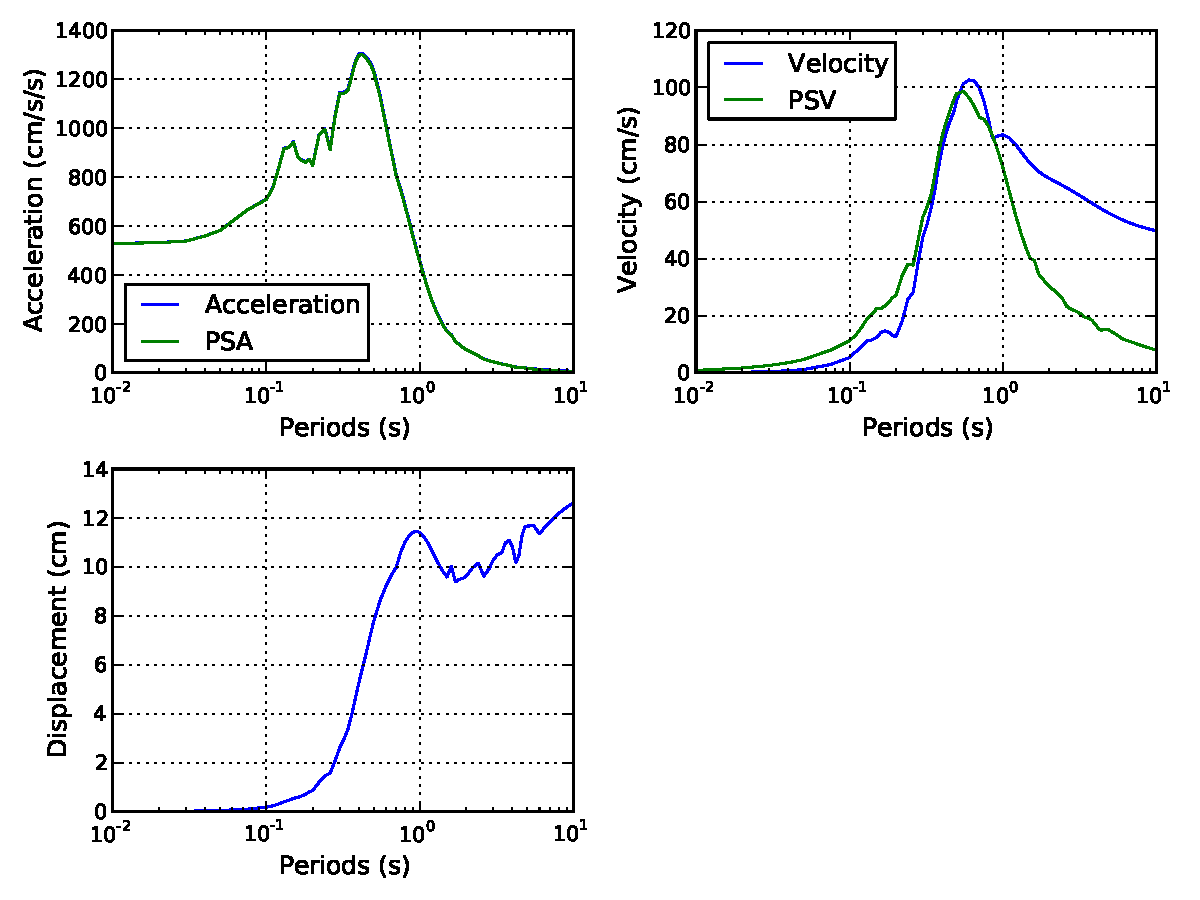
\includegraphics[width=\textwidth]{./figures/ims/response_newmark_beta.pdf}
	\caption{Full response spectra of the waveform shown in Figure \ref{fig:time_series}, calculated using the Newmark-$\beta$ method}
	\label{fig:newmark_beta}
\end{figure}
\begin{figure}[htb]
	\centering
		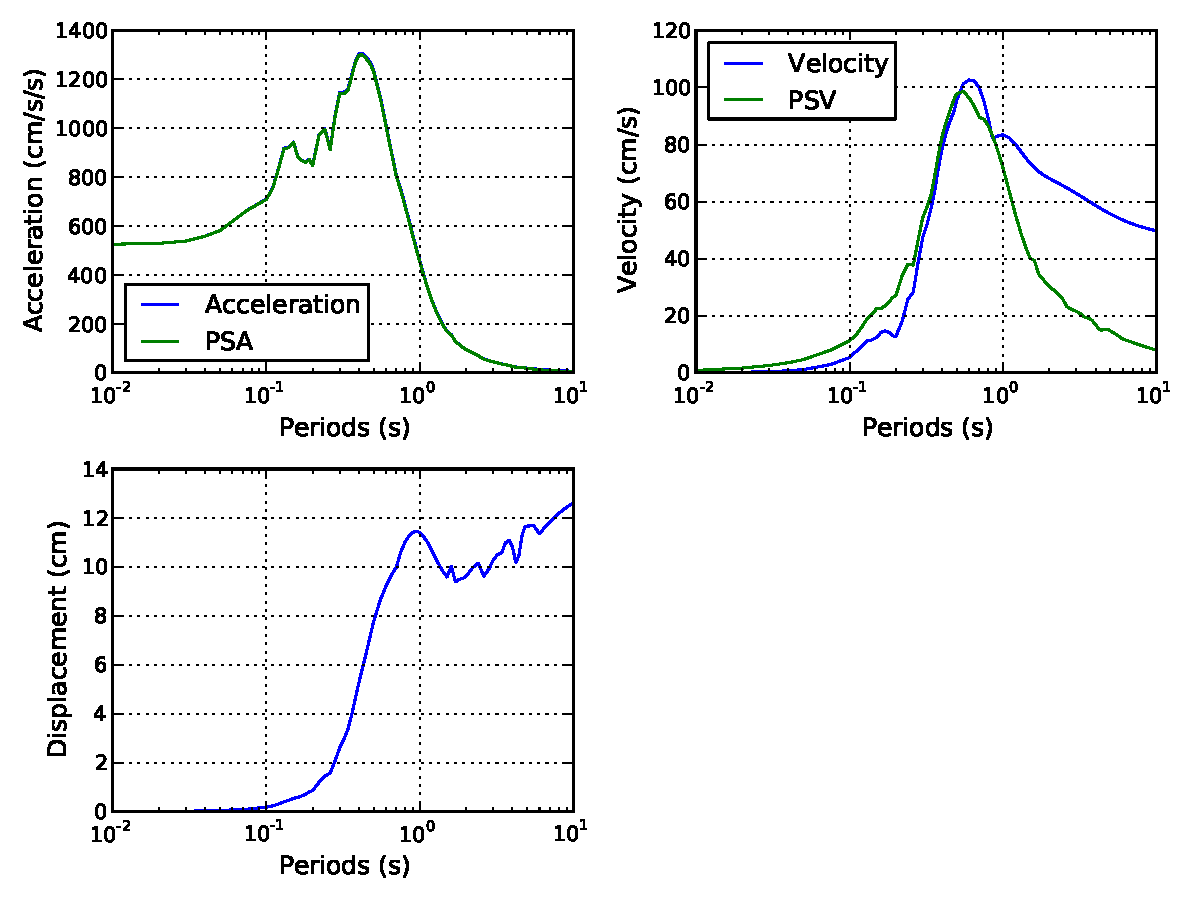
\includegraphics[width=\textwidth]{./figures/ims/response_nigam_jennings.pdf}
	\caption{Full response spectra of the waveform shown in Figure \ref{fig:time_series}, calculated using the Nigam \& Jennings (1969) method}
	\label{fig:nigam_jennings}
\end{figure}

\noindent where \verb=spectra= is the response spectra dictionary, \verb=axis_type= defines the type of axes: ``loglog'' (double logarithmic - the default), ``semilogx'' (logarithmic period axis), ``semilogy'' (logarithmic spectral response axis), ``linear'' (both axes linear). The function also takes the same keywords as the \verb=plot_time_series= method, i.e. \verb=figure_size=, \verb=filename=, \verb=filetype=, \verb=dpi=.

It can be seen from Figures  \ref{fig:newmark_beta} and \ref{fig:nigam_jennings} that both methods give very similar results.

\section{Combining Horizontal Components of Motion}
\label{sec:horizontal}

For a pair of horizontal records it is necessary to define a spectrum representing the ``horizontal'' component of ground motion. The manner in which the two horizontal components of motion are resolved can be treated in many different ways \citep[e.g.][]{Douglas2003, BeyerBommer2006}. The intensity measure tools contain various methods for combining horizontal response spectra. 

The first step in the application of these methods may be to extract the respective response spectra for the two horizontal components. This can be done as follows:

\begin{python}[frame=single]
spectra_x, spectra_y = ims.get_response_spectrum_pair(
    accel_x,
    time_step, # Time-step of x-component
    accel_y,
    time_step, # Time-step of y-component,
    periods,
    damping=0.05,
    units="cm/s/s",
    method="Nigam-Jennings")
\end{python}

In the case of the records demonstrated the time-step is the same for both horizontal components. If it is not the same, however, the response spectra can still be calculated.

Given the pair of records, \verb=spectra_x= ($Sa_x \left( {T, \xi} \right)$)and \verb=spectra_y= ($Sa_y \left( {T, \xi} \right)$), we can now obtain the following ``resolved'' horizontal spectra:

\begin{itemize}
\item \textbf{Geometric Mean}
    \begin{equation}
    Sa_{gm} \left( {T, \xi} \right) = \sqrt{Sa_x \left( {T, \xi} \right) \times Sa_y \left( {T, \xi} \right)}
    \end{equation}
    Calculated using the following command:
    \begin{python}
sa_gm = ims.geometric_mean_spectrum(spectra_x, spectra_y)
    \end{python}
    
\item \textbf{Arithmetic Mean}
    \begin{equation}
    Sa_{am} \left( {T, \xi} \right) = \frac{1}{2} \left( {Sa_x \left( {T, \xi} \right) + Sa_y \left( {T, \xi} \right)} \right)
    \end{equation}  
        Calculated using the following command:
    \begin{python}
sa_am = ims.arithmetic_mean_spectrum(spectra_x, spectra_y)
    \end{python}  

\item \textbf{Larger PGA}
    This simply returns the spectrum of the time series that gives the largest spectral acceleration. Calculated using the following command:
    \begin{python}
sa_larger = ims.larger_pga(spectra_x, spectra_y)
    \end{python}   

\item \textbf{Envelope}
    This returns a spectrum representing the larger of the two components for each period such that:
    \begin{equation}
    Sa_{env} \left( {T_i, \xi} \right) = \max\left( {Sa_x \left( {T_i, \xi} \right), Sa_y \left( {T_i, \xi} \right)} \right) \quad \text{for} \quad i = 1, 2, \ldots, N_{PERIODS}  
    \end{equation}
    \begin{python}
sa_env = ims.envelope(spectra_x, spectra_y)
    \end{python}  
\end{itemize}

In each of these cases the output of the function is a dictionary containing the same keys as that of the \verb=spectra=, but with the resolved horizontal values of each of the quantities. 

For the two spectra considered here, the geometric mean spectra and the envelope spectra are shown in Figures \ref{fig:geometric} and \ref{fig:envelope} respectively. 

\begin{figure}[htb]
	\centering
		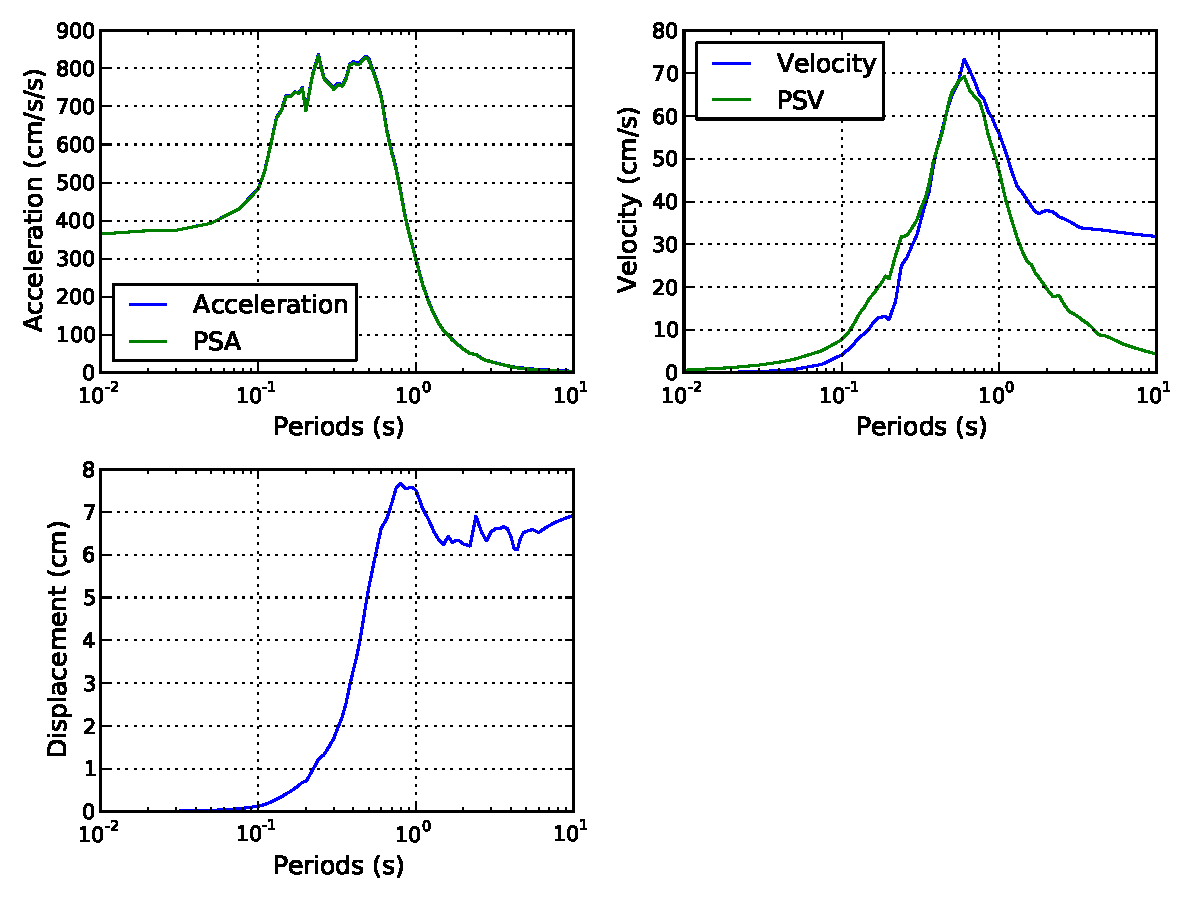
\includegraphics[width=12cm]{./figures/ims/geometric_mean_spectrum.pdf}
	\caption{Geometric mean spectra of the two horizontal records}
	\label{fig:geometric}
\end{figure}
\begin{figure}[htb]
	\centering
		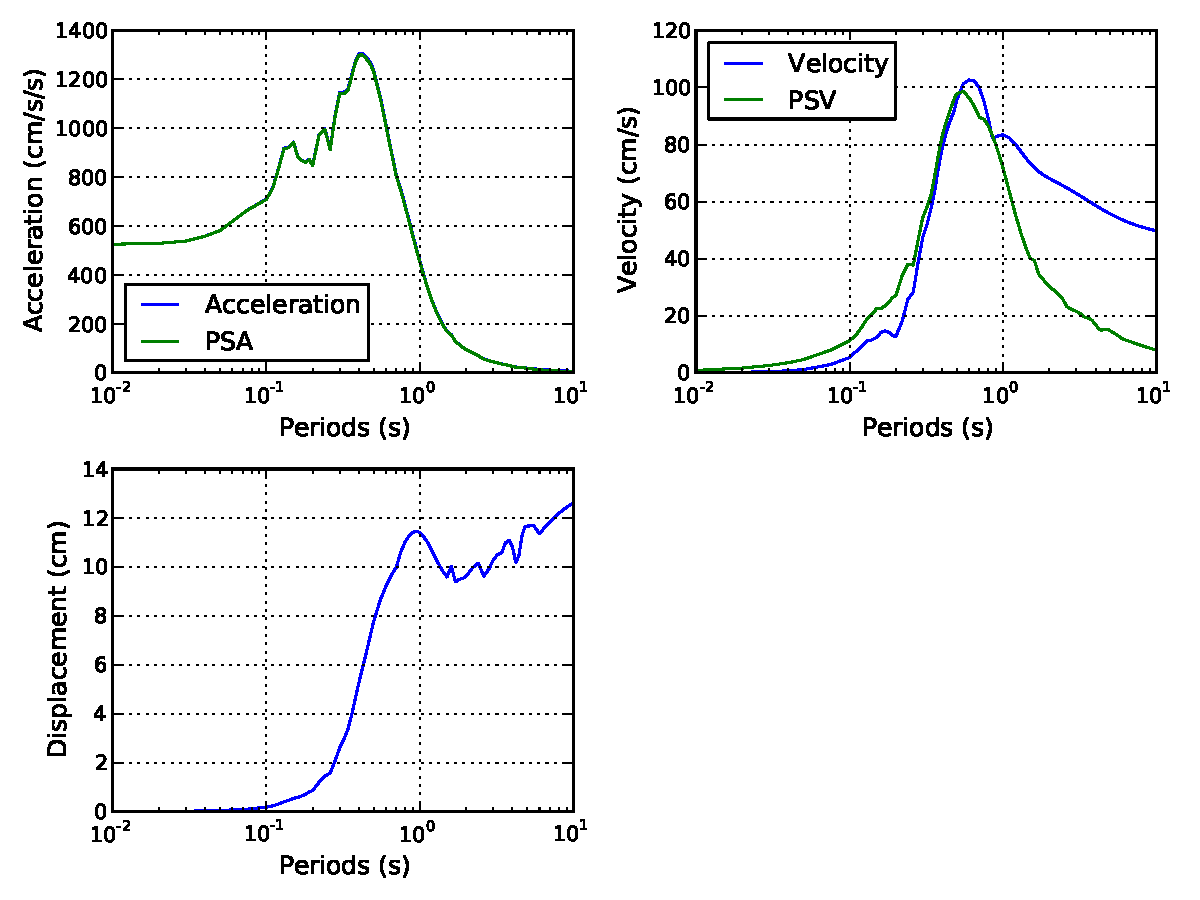
\includegraphics[width=12cm]{./figures/ims/envelope_spectrum.pdf}
	\caption{Envelope spectra of the two horizontal records}
	\label{fig:envelope}
\end{figure}

\section{Rotation of the Horizontal Records}

In some applications it may be necessary to rotate a pair of horizontal time series, either to orient them into fault-normal and fault-parallel components, or to some direction that may represent the most adverse for a particular structure. For two time series of equal duration and time series, the records can be rotated through angle $\theta$:

\begin{equation}
\begin{pmatrix}a_{x \left( {\theta} \right)} \left( t \right) \\ a_{y \left( {\theta} \right)} \left( t \right)\end{pmatrix} = \begin{bmatrix}\cos \theta & \sin \theta \\ -\sin \theta & \cos \theta \end{bmatrix} \begin{pmatrix}a_x\left( t \right) \\ a_y\left( t \right)\end{pmatrix}
\end{equation}

\noindent This can be achieved using the \verb=ims= tools:

\begin{python}[frame=single]
rot_hist_x, rot_hist_y = ims.rotate_horizontal(accel_x,
                                               accel_y,
                                               theta)
\end{python}

The incorporation of rotational tools permits the toolkit to calculate the ``orientation-dependent'' and ``orientation-independent'' geometric mean of a horizontal pair of records, as described in detail in \cite{Boore_etal2006}. The two quantities, \verb=GMRotDpp= and \verb=GMRotIpp= respectively, cannot be calculated from the two horizontal response spectra directly as other horizontal measures are. As they require rotation of time-series through non redundant angles, it is necessary to determine the response spectra for each rotation angle.

To calculate \verb=GMRotDpp= and \verb=GMRotIpp= run:

\begin{python}
gmrotd50 = ims.gmrotdpp(accel_x, time_step,
                        accel_y, time_step,
                        periods,
                        50.0, # Percentile
                        damping=0.05,
                        units="cm/s/s",
                        method="Nigam-Jennings")
gmroti50 = ims.gmrotipp(accel_x, time_step,
                        accel_y, time_step,
                        periods,
                        50.0, # Percentile
                        damping=0.05,
                        units="cm/s/s",
                        method="Nigam-Jennings")
\end{python}


\section{Adding Horizontal Components to the Database}

In the process of constructing the database of strong motion records it may often be prudent to compile the database in steps, of which the final one may often be the addition of the resolved horizontal components of the strong motion record. Depending on the data, and the required intensity measures, the calculation of horizontal spectra may be a (relatively) slow process with respect to the rest of the database construction. It is recommended that the database be constructed in the manner described in section \ref{sec:hdf5}, and then the resolved horizontal components added subsequently. To facilitate this a function is added to the database builder, which will add the desired horizontal ground motions to an existing database. An example is seen below:

\begin{python}[frame=single]
# Import the function add_horizontal_im
from smtk.sm_database_buider import add_horizontal_im
# Load in the database metadata file
import cPickle
database = cPickle.load(open("path/to/metadata.pkl", "r"))
# Choose the desired horizontal intensity measures
# The following will add the horizontal PGA, PGV
# Geometric mean spectrum, envelope spectrum and GMRotI50
im_list = ["PGA", "PGV", "Geometric", "Envelope", "GMRotI50"]
add_horizontal_im(database,
                  im_list, 
                  component="Geometric",
                  damping="05",
                  periods=[])
\end{python}

Depending on the size of the database this may take \textbf{many hours} to run (especially if rotational parameters are required). In this function the keyword \verb=component= refers only to the horizontal component of the scalar values. For the spectra, the type of horizontal component should be given in the intensity measure list. Note also that unlike the \verb=ims= and \verb=rsp= tools in which the damping is input as a floating point value, here it is input as a string. If not input by the user, the periods will be taken from the values stored in the x-component of the record. 

